%%%%%%%%%%%%%%%%%%%%%%%%%%%%%%%%%%%%%%%%%%%%%%%%%%%%%%%%%%%%%%%%%%%%%%
% Overleaf (WriteLaTeX) Example: Molecular Chemistry Presentation
%
% Source: http://www.overleaf.com
%
% In these slides we show how Overleaf can be used with standard 
% chemistry packages to easily create professional presentations.
% 
% Feel free to distribute this example, but please keep the referral
% to overleaf.com
% 
%%%%%%%%%%%%%%%%%%%%%%%%%%%%%%%%%%%%%%%%%%%%%%%%%%%%%%%%%%%%%%%%%%%%%%
% How to use Overleaf: 
%
% You edit the source code here on the left, and the preview on the
% right shows you the result within a few seconds.
%
% Bookmark this page and share the URL with your co-authors. They can
% edit at the same time!
%
% You can upload figures, bibliographies, custom classes and
% styles using the files menu.
%
% If you're new to LaTeX, the wikibook is a great place to start:
% http://en.wikibooks.org/wiki/LaTeX
%
%%%%%%%%%%%%%%%%%%%%%%%%%%%%%%%%%%%%%%%%%%%%%%%%%%%%%%%%%%%%%%%%%%%%%%

\documentclass{beamer}

% For more themes, color themes and font themes, see:
% http://deic.uab.es/~iblanes/beamer_gallery/index_by_theme.html
%
\mode<presentation>
{
  \usetheme{Madrid}       % or try default, Darmstadt, Warsaw, ...
  \usecolortheme{default} % or try albatross, beaver, crane, ...
  \usefonttheme{serif}    % or try default, structurebold, ...
  \setbeamertemplate{navigation symbols}{}
  \setbeamertemplate{caption}[numbered]
} 

\usepackage[english]{babel}
\usepackage[utf8x]{inputenc}
\usepackage{chemfig}
\usepackage[version=3]{mhchem}

% On Overleaf, these lines give you sharper preview images.
% You might want to `comment them out before you export, though.
\usepackage{pgfpages}
\pgfpagesuselayout{resize to}[%
  physical paper width=8in, physical paper height=6in]

%==================================
\usepackage{subfigure}
%==================================

% Here's where the presentation starts, with the info for the title slide
\title[My Computer Graphics Background]{A short presentation on my background in computer graphics}
\author{M. Mostajab}
\institute{www.mmostajab.com}
\date{\today}

\begin{document}

\begin{frame}
  \titlepage
\end{frame}

% These three lines create an automatically generated table of contents.
\begin{frame}{Outline}
  \tableofcontents
\end{frame}

\section{Introduction}

\begin{frame}{About Me...}
	\begin{tikzpicture}[overlay, remember picture]
		\node[anchor=north east, xshift=-40pt,yshift=-55pt]
		at(current page.north east){
			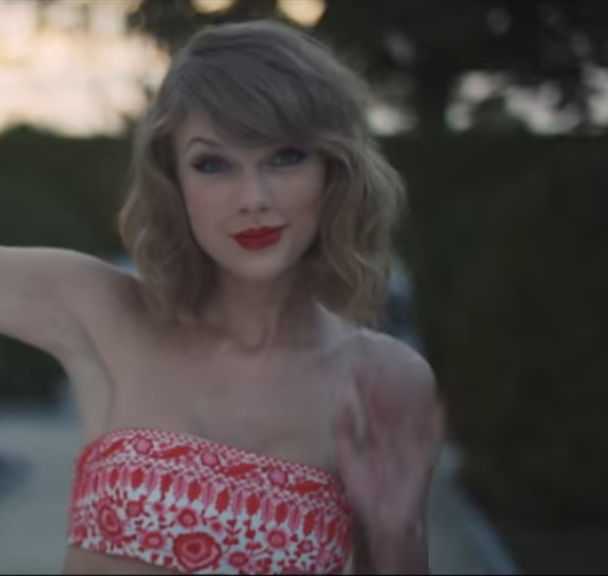
\includegraphics[width=30mm]{figures/FirstPC.png}
		};
	\end{tikzpicture}

	\begin{itemize}
		\item My name is \textbf{Morteza Mostajab}
		\item Bachelor studies:\\ Hamedan University of Technology, Iran
		\item Maseter studies:\\ Technische Universit{\"a}t M{\"unchen}
		\item Present:\\ Researcher at Fraunhofer IGD, Darmstadt
		\item Research interests:\\
		    Real-time physically-based rendering \\
		    (Rasterization-based or Ray-tracing)\\
			Virtual reality\\
			Computer graphics and visualization\\
			Game Programming
		   
	\end{itemize}
\end{frame}

\begin{frame}{Inspiration}
	
	\begin{itemize}
		\item Games, Animations, Movies with Special Effects,...
			\begin{figure}
			\centering
			\subfigure[Lion King]{
				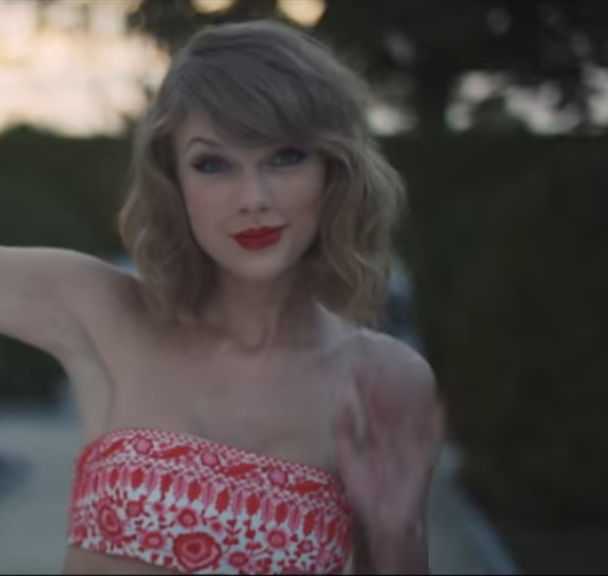
\includegraphics[width=0.22\linewidth]{figures/Inspiration1.png}
			}
			\subfigure[caption]{
				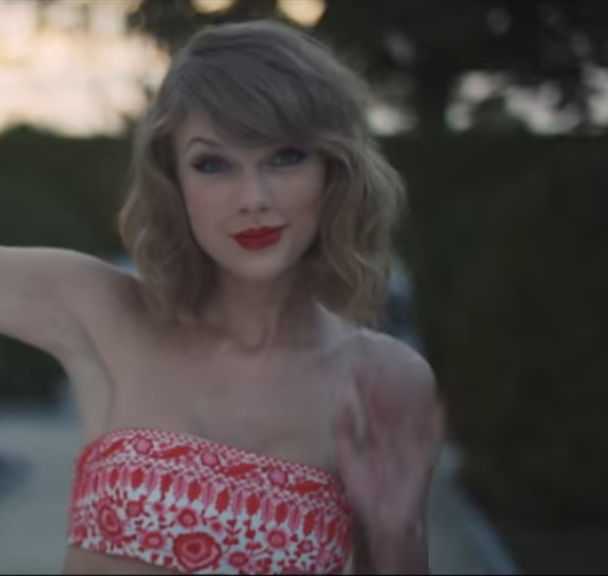
\includegraphics[width=0.22\linewidth]{figures/Inspiration1.png}
			}
		\end{figure}
	  \item My firsts...
		  \begin{figure}
			\centering
			\subfigure[First Computer]{
				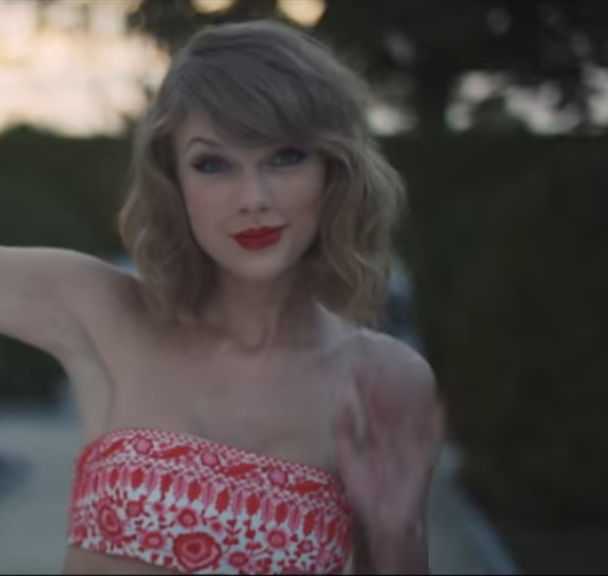
\includegraphics[height=0.2\textheight]{figures/FirstComputer.png}
			}
			\subfigure[First PC]{
				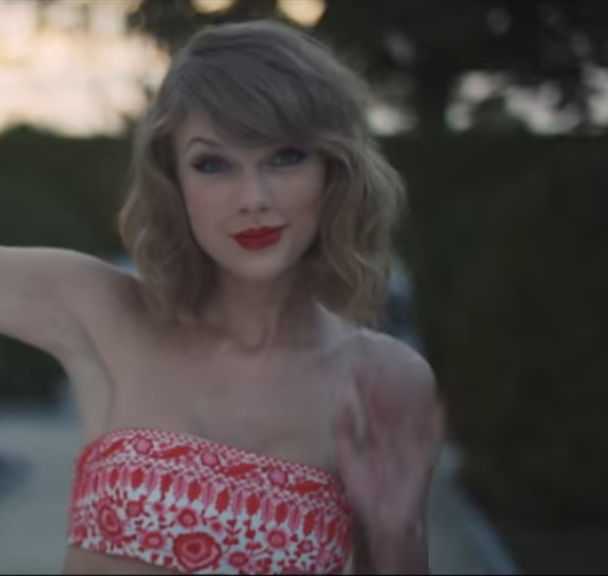
\includegraphics[height=0.2\textheight]{figures/FirstPC.png}
			}
			\subfigure[First Console]{
				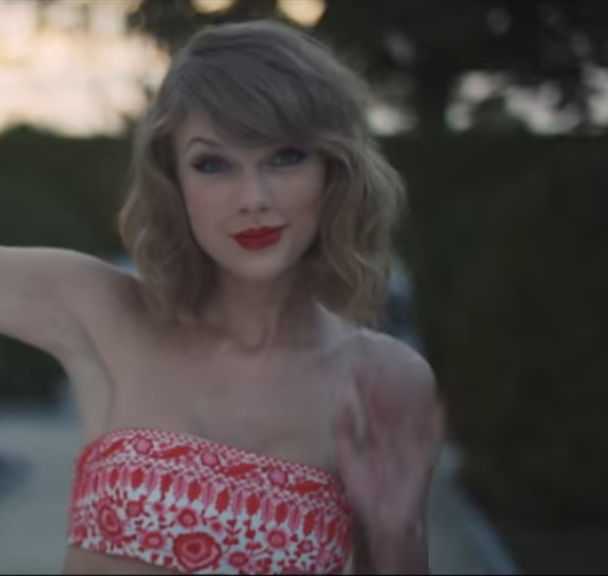
\includegraphics[height=0.2\textheight]{figures/FirstConsole.png}
			}
       	  \end{figure} 
	\end{itemize}
\end{frame}

\section{Master Thesis}

\section{Ray tracing revisited for rendering CSG models consisting of higher order primitives}


\begin{frame}{Inspiration}
	
	\begin{itemize}
		\item In these slides we show how Overleaf can be used with standard chemistry packages to easily create professional presentations.
		\item If you're new to \LaTeX{}, check out this free introductory course by Overleaf founder Dr John Lees-Miller: \url{www.overleaf.com/blog/7}
		\item You can also find more quick tips and tricks on the help pages at \url{www.overleaf.com/help}
	\end{itemize}

% Example from Chemfig documentation - Fischer indole synthesis:
% www.tex.ac.uk/ctan/macros/generic/chemfig/chemfig_doc_en.pdf
\begin{center}\small\setatomsep{1.5em}
\schemestart
  \chemfig{*6(=-*6(-\chembelow{N}{H}-NH_2)=-=-)}
  \+
  \chemfig{(=[:-150]O)(-[:-30]R_2)-[2]-[:150]R_1}
  \arrow(.mid east--.mid west){->[\chemfig{H^+}]}
  \chemfig{*6(-=*5(-\chembelow{N}{H}-(-R_2)=(-R_1)-)-=-=)}
\schemestop
\end{center}

\end{frame}

\subsection{The chemistry packages}
\begin{frame}{The chemistry packages}

We focus on two \LaTeX{} chemistry packages:
\begin{block}{The \texttt{chemfig} package}
This package provides the command which draws molecules. Created by Christian Tellechea, a detailed user guide can be found here:\\[0.4cm]
\small{\url{www.tex.ac.uk/ctan/macros/generic/chemfig/chemfig_doc_en.pdf}}
\end{block}
\begin{block}{The \texttt{mhchem} package}
The \texttt{mhchem} package provides simple commands for typesetting chemical molecular formulae and equations. Created by Martin Hensel, a detailed user guide can be found here:\\[0.4cm]
\small{\url{http://mirror.ox.ac.uk/sites/ctan.org/macros/latex/contrib/mhchem/mhchem.pdf}}
\end{block}
% The LaTeX wikibook is also a good source of info, e.g.
% http://en.wikibooks.org/wiki/LaTeX/Chemical_Graphics

\end{frame}

\end{document}